\documentclass[tikz]{beamer}

\usepackage{tikz}
\usetikzlibrary{shapes,arrows}
\mode<presentation>{}
\usepackage{beamerthemeshadow}

%\usepackage{pseudocode}
%\usepackage{dirtree}
% \usepackage[utf8]{inputenc}
% \usepackage{listings,xcolor}

% \usepackage{soul}
% \usepackage{ulem}


\usepackage{tikz-cd}
\usepackage{amsmath}
\usepackage[most]{tcolorbox}


\DeclareMathOperator*{\argmin}{arg\,min}


\usepackage[linesnumbered,lined,boxed,commentsnumbered]{algorithm2e}
%\usepackage{algorithmicx}
\usepackage{algpseudocode}
\algrenewcommand\algorithmicwhile{\textbf{until}}
\SetKwInOut{Input}{input}
\SetKwInOut{Output}{output}



\usepackage[round,authoryear]{natbib}
%\usepackage[margin=1.0in]{geometry}
\usepackage{graphicx}
\usepackage{moreverb}
\usepackage{hyperref}
\newcommand\infNorm[1]{\left\lVert#1\right\rVert_\infty}
\newcommand\twoNorm[1]{\left\lVert#1\right\rVert_2}
\newcommand\someNorm[1]{\left\lVert#1\right\rVert}

\usepackage{mathtools}
\mathtoolsset{showonlyrefs}

\usepackage[english]{babel}
\usepackage[12hr,level]{datetime}
%\usepackage{datetime}
\usepackage{amsfonts}

\newcommand{\xgusst}[1]{x^{guess}_{#1}}
\newcommand{\xnxt}[1]{x^{next}_{#1}}
\newcommand{\znxt}[1]{z^{next}_{#1}}
\newcommand{\xlst}[1]{x^{last}_{#1}}
\newcommand{\zlst}[1]{z^{last}_{#1}}
\newcommand{\zgusst}[1]{z^{guess}_{#1}}
\newcommand{\xguss}{\xgusst{}}
\newcommand{\xtpguss}{x^{tp1guess}}


\newcommand{\iSet}{{\mathcal{I}_t}}

\newcommand{\posInt}{{\mathcal{N}^+}}
\newcommand{\Rn}[1]{{\mathcal{R}^{#1}}}
\newcommand{\numX}{{N_x}}
\newcommand{\numZ}{{N_z}}
\newcommand{\numEps}{{N_\epsilon}}
\newcommand{\numR}{{N_r}}
\newcommand{\numIters}{{K}}
\newcommand{\numTerms}{{N_{terms}}}
\newcommand{\numPts}{{N_{points}}}
\newcommand{\thePoints}{{\{(x_{t-1},\epsilon_t)^{1} \ldots (x_{t-1},\epsilon_t)^{\numPts}\}}}
\newcommand{\thePts}{{\mathcal{P}}}
%\newcommand{\ADRCE}{{\bf ADRCE}}
%\newcommand{\ADR}{{\bf ADR}}
\newcommand{\ADRCE}{\XZFunc}
\newcommand{\ADR}{\xzFunc}




\newcommand{\xtmEpsArg}{{x_{t-1},\epsilon_t}} 
\newcommand{\xtArg}{{x_{t} }}


\newcommand{\sumLinPart}{{
B x_{t-1}+ \phi \psi_\epsilon\epsilon + (I - F)^{-1} \phi \psi_c 
}}
\newcommand{\sumZPart}{{
 \sum_{\sForSum=0}^\infty F^s \phi z_{t+\sForSum}(x_{t-1},\epsilon) 
}}
\newcommand{\sumZPartZero}{{
 \phi z_{t}(x_{t-1},\epsilon) 
}}
\newcommand{\sumZPartPos}{{
 \sum_{\sForSum=1}^\infty F^s \phi Z_{t+\sForSum}(x_{t-1},\epsilon) 
}}

\newcommand{\EsumLinPart}{{
	 B x_{t-1}+ (I - F)^{-1} \phi \psi_c 
}}
\newcommand{\EsumZPartZero}{{
	  \sum_{\sForSum=0}^\infty F^s \phi Z^{PF}_{t+\sForSum}(x_{t-1},0) 
}}
\newcommand{\EsumZPartEpsilon}{{
	  \sum_{\sForSum=0}^\infty F^s \phi \expct{z_{t+\sForSum}(x_{t-1},\epsilon)}
}}
\newcommand{\EsumCapZPart}[1]{{
	  \sum_{\sForSum=0}^\infty F^s \phi {Z^{#1}_{t+\sForSum}(x_{t-1})}
}}
\newcommand{\uncnxpt}[2]{{\mathcal{E}\left [ \left . #1 \right | #2  \right ]}}
\newcommand{\expct}[1]{{\mathcal{E}\left [ #1 \right ]}}

\newcommand{\xzFuncGuess}{{\mathbb{g}}}
\newcommand{\xzFuncGuessIn}{{\mathbf{\mathbb{g}_{in}}}}
\newcommand{\genxzFuncGuessIn}{{\mathbf{gen\mathbb{g}_{in}}}}
\newcommand{\xzFuncGuessSig}{{(\Rn{\numX})\rightarrow
(\Rn{({\numX+\numZ})})}}


\newcommand{\xzFunc}{{{\gamma}}}
\newcommand{\xzFuncSig}{{(\Rn{\numX+\numEps})\rightarrow
(\Rn{({\numX+\numZ})})}}

\newcommand{\XZFunc}{{\mathbb{G}}}
\newcommand{\genXZFunc}{{\mathbf{gen\mathbb{G}}}}
\newcommand{\bigXFuncSig}{{(\Rn{\numX})\rightarrow
(\Rn{({\numX+\numZ})})}}


\newcommand{\genXGFP}{{\mathcal{U}}}
\newcommand{\xgFP}{{\mathcal{V}}}

\newcommand{\genFpf}{{\mathbf{gen}_\fpf}}
\newcommand{\fpf}{{\mathcal{T}}}
\newcommand{\fpfIn}{{\mathbf{t}_{in}}}
\newcommand{\fpfOut}{{\mathbf{t}_{out}}}
\newcommand{\genFpfIn}{{\mathbf{gen\fpf}_{in}}}
\newcommand{\genFpfOut}{{\mathbf{gen\fpf}_{out}}}

\newcommand{\genSlvr}{{\mathbf{gen}_{\slvr}}}
\newcommand{\slvr}{{\mathcal{S}}}
\newcommand{\slvrIn}{{\mathbf{s}_{in}}}
\newcommand{\slvrOut}{{\mathbf{s}_{out}}}
\newcommand{\genSlvrIn}{{\mathbf{gen\slvr}_{in}}}
\newcommand{\genSlvrOut}{{\mathbf{gen\slvr}_{out}}}
\newcommand{\solverSig}{{
\frfpnsRegimeFuncHelp
}}
\newcommand{\allArgs}{(x_{t-1},\epsilon,x_t,\expct{x_{t+1}})}
\newcommand{\proj}[1]{{\pi_{#1}}}
\newcommand{\eqnArg}{\mathbf{m}_{in}}
\newcommand{\eqnOut}{\mathbf{m}_{err}}
\newcommand{\eqnFunc}{\mathbb{M}}
\newcommand{\gate}{\mathbf{b}}
\newcommand{\eqnFuncSysIExpl}[1]{\{(\mathbf{b}_{#1}\allArgs,\eqnFunc_{#1}\allArgs=0) \}}
\newcommand{\eqnFuncSysI}[1]{\mathbb{C}_{#1}}
\newcommand{\eqnFuncSys}{\{\eqnFuncSysI{1},\ldots,\eqnFuncSysI{M}\}}
\newcommand{\eqnErrs}{{{m}_e}}
\newcommand{\eqnFuncSig}{{\Rn{3\numX+\numEps+\numZ}\rightarrow\Rn{\numX}}}


\newcommand{\lilXFuncSig}{{fix lilXFuncSig}}



\newcommand{\frfpnsFuncSig}{{\Rn{\numX+\numEps}\rightarrow\Rn{\numX+\numZ}}}

\newcommand{\bigXRegimeFuncSig}{{(\Rn{\numX+1})\rightarrow
(\Rn{({\numX+\numZ})})}}
\newcommand{\lilXRegimeFuncSig}{{(\Rn{\numX+1+\numEps+\numZ})\rightarrow
(\Rn{({3(\numX+1)+\numEps+\numZ})})}}
\newcommand{\eqnRegimeFuncSig}{{
\{\Rn{3(\numX+1)+\numEps+\numZ}\rightarrow\Rn{\numX},
\ldots,
\Rn{3(\numX+1)+\numEps+\numZ}\rightarrow\Rn{\numX}\}
}}
\newcommand{\frfpnsRegimeFuncHelp}{{\Rn{\numX+\numEps}\rightarrow\Rn{\numX+\numZ}}}

\newcommand{\frfpnsRegimeFuncSig}{{
\{ (\frfpnsRegimeFuncHelp{1}), \ldots ,  (\frfpnsRegimeFuncHelp{\numR})\}
}}

\newcommand{\dstSpec}{{\mathbf{distSpec}}}
\newcommand{\expctSpec}{{\mathbf{expctSpec}}}
\newcommand{\grdSpec}{{\mathbf{grdSpec}}}


\newcommand{\linMod}{{\mathcal{L}}}
\newcommand{\linModMats}{{\{H,\psi_\epsilon,\psi_c;B,\phi,F\}}}
\newcommand{\sForSum}{{\nu}}

\newcommand{\xWOarg}{   \mathbf{x}}
\newcommand{\xWarg}{   \mathbf{x}(x_{t-1},\epsilon)}
\newcommand{\xWargK}{   \hat{\mathbf{x}}(x_{t-1},\epsilon,k)}
\newcommand{\xWOargK}{   \hat{\mathbf{x}}}

\newcommand{\xpWOarg}{   \mathbf{x}^p}
\newcommand{\xpWarg}{   \mathbf{x}^p(x_{t-1},\epsilon)}
\newcommand{\xpWargK}{   \hat{\mathbf{x}}^p(x_{t-1},\epsilon,k)}
\newcommand{\xpWOargK}{   \hat{\mathbf{x}^p}}


\newcommand{\xppWOarg}{   \mathbf{x}^{p'}}
\newcommand{\xppWarg}{   \mathbf{x}^{p'}(x_{t-1},\epsilon)}
\newcommand{\xppWargK}{   \hat{\mathbf{x}}^{p'}(x_{t-1},\epsilon,k)}
\newcommand{\xppWOargK}{   \hat{\mathbf{x}^{p'}}}



\newcommand{\XWOarg}{   \mathbf{X}}
\newcommand{\XWarg}{   \mathbf{X}(x_{t-1},\epsilon)}
\newcommand{\XWargK}{   \hat{\mathbf{X}}(x_{t-1},\epsilon,k)}
\newcommand{\XWOargK}{   \hat{\mathbf{X}}}


\newcommand{\XpWOarg}{   \mathbf{X}^p}
\newcommand{\XpWarg}{   \mathbf{X}^p(x_{t-1},\epsilon)}
\newcommand{\XpWargK}{   \hat{\mathbf{X}^p}(x_{t-1},\epsilon,k)}
\newcommand{\XpWOargK}{   \hat{\mathbf{X}^p}}

\newcommand{\zWOarg}{   \mathbf{z}}
\newcommand{\zWarg}{   \mathbf{z}(x_{t-1},\epsilon)}
\newcommand{\zWargK}{   \hat{\mathbf{z}}(x_{t-1},\epsilon,k)}
\newcommand{\zWOargK}{   \hat{\mathbf{z}}}


\newcommand{\ZWOarg}{   \mathbf{Z}}
\newcommand{\ZWarg}{   \mathbf{Z}(x_{-1},\epsilon)}
\newcommand{\ZWargK}{   \hat{\mathbf{Z}}(x_{-1},\epsilon,k)}
\newcommand{\ZWOargK}{   \hat{\mathbf{Z}}}


\newcommand{\zpWOarg}{   \mathbf{z}^p}
\newcommand{\zpWarg}{   \mathbf{z}^p(x_{t-1},\epsilon)}
\newcommand{\zpWargK}{   \hat{\mathbf{z}^p}(x_{t-1},\epsilon,k)}
\newcommand{\zpWOargK}{   \hat{\mathbf{z}^p}}



\newcommand{\zppWOarg}{   \mathbf{z}^{p'}}
\newcommand{\zppWarg}{   \mathbf{z}^{p'}(x_{t-1},\epsilon)}
\newcommand{\zppWargK}{   \hat{\mathbf{z}^{p'}}(x_{t-1},\epsilon,k)}
\newcommand{\zppWOargK}{   \hat{\mathbf{z}^{p'}}}


\newcommand{\ZpWOarg}{   \mathbf{Z}^p}
\newcommand{\ZpWarg}{   \mathbf{Z}^p(x_{-1},\epsilon)}
\newcommand{\ZpWargK}{   \hat{\mathbf{Z}^p}(x_{-1},\epsilon,k)}
\newcommand{\ZpWOargK}{   \hat{\mathbf{Z}^p}}


\newcommand{\xIter}[2]{\mathcal{X}^{#1}(#2)}
\newcommand{\xNow}[1]{x^{#1}_t(x_{t-1},\epsilon_t)}
\newcommand{\zNow}[1]{z^{#1}(x_{t-1},\epsilon_t)}
\newcommand{\xNowtp}[1]{x^{#1}_{t+1}(x_{t-1},\epsilon_t)}
\newcommand{\XNow}[3]{\mathcal{X}^{#1}_{#2}(x_{#3})}
\newcommand{\ZNow}[3]{\mathcal{Z}^{#1}(x_{#3})}


\newcommand{\rcpC}{{\mathbf{N}}}


\newcommand{\gssaKtp}{{\left \{  
\beta \frac{u^\prime(c_{\tau+1})}{u^\prime(c_{\tau})} 
[1- \delta + a_{t+1}f^\prime(k_{\tau+1})]
\right \} -1}}


\newenvironment{myProof}[1][Proof]{\begin{trivlist}
  \item[\hskip \labelsep {\bfseries #1}]}{\end{trivlist}}
\newenvironment{myDefinition}[1][Definition]{\begin{trivlist}
\item[\hskip \labelsep {\bfseries #1}]}{\end{trivlist}}
\newenvironment{myExample}[1][Example]{\begin{trivlist}
\item[\hskip \labelsep {\bfseries #1}]}{\end{trivlist}}
\newenvironment{myRemark}[1][Remark]{\begin{trivlist}
\item[\hskip \labelsep {\bfseries #1}]}{\end{trivlist}}

\newcommand{\myQed}{\nobreak \ifvmode \relax \else
      \ifdim\lastskip<1.5em \hskip-\lastskip
      \hskip1.5em plus0em minus0.5em \fi \nobreak
      \vrule height0.75em width0.5em depth0.25em\fi}

\newcommand{\xtFuncTI}{\mathcal{X}(x,\epsilon)}
\newcommand{\XtFuncTI}{\mathbf{X}(x)}
\newcommand{\expctEps}[1]{\mathcal{E}_{\epsilon} \left [#1 \right ]}
\newcommand{\xsubtFunc}[2]{\mathcal{X}_{#1}{#2}}
\newcommand{\xtFunc}[1]{\mathcal{X}{#1}}
\newcommand{\XtFunc}[1]{\mathbf{X}{#1}}
\newcommand{\stochF}[1]{\mathcal{S}^{\{#1\}}}
\newcommand{\detF}[1]{\mathcal{D}^{\{#1\}}}
\newcommand{\initXE}{(x_{-1},\epsilon_0)}
\newcommand{\nlEqnLHS}[4]{
  h_\varpi(#1,#2,E_t(#3),\epsilon_#4)}

\newcommand{\nlEqn}[4]{
h_\varpi^{det}(#1,#2,\epsilon_#4)+
H_\varpi^{det}(#1,#2,\epsilon_#4)E_#4(#3)
}
\newcommand{\nlEqnSel}[4]{
\varpi=m_\varpi^{det}(#1,#2,\epsilon_#4)+
M_\varpi^{det}(#1,#2,\epsilon_#4)E_#4(#3)
}
\newcommand{\itSup}[1]{{\{#1\}}}
\newcommand{\initX}{(x)}
\newcommand{\initXEN}{(x_,\epsilon_t)}
\newcommand{\detComp}[1]{{\detF{K-\nu}( \cdots \detF{K-1}(\detF{K}(#1))))}}
\newcommand{\tArg}{(x_{t-1},\epsilon_t)}
\newcommand{\tNo}{(x_{t-1})}


\newtheorem{theorem}{Theorem}[section]


\newcommand{\fSum}{\mathcal{F}}
\newcommand{\modArgs}{\mathbb{X}}

\newcommand{\aSmolPoly}{p(x,\epsilon)}
\newcommand{\smolRngs}{\{(\underbar{x}_1,\bar{x}_1),\ldots,(\underbar{x}_L,\bar{x}_L),(\underbar{$\epsilon$}_1,\bar{\epsilon}_1),\ldots,(\underbar{$\epsilon$}_L,\bar{\epsilon}_K)\}}
\newcommand{\distribSpec}{\{f_1,\ldots,f_K\}}


%
\newcommand{\eulerE}{\mathbf{e}}

\begin{document}
\title[A Series Representation  for Solving  Models]{A Series Representation for Dynamic Economic Model Solutions: Regime Switching DSGE Models with Occasionally Binding Constraints }
%\subtitle{this is a subtitle}


\author{Gary S. Anderson}
\date{June 26, 2016} 


\frame{\titlepage}

\section{Introduction and Summary}

\begin{frame}

 \begin{itemize}
 \item Proposing a series representation for a broad class of functions
 \item Easy to compute representation for representing
families of trajectories
\item only requires that the trajectories are bounded
\item originally motivated by solving models occassionally binding constraints
\item series representation seems much more general flexible than I originally imagined
\end{itemize}
\end{frame}


\begin{frame}
     \begin{itemize}
   \item Today focus on time invariant decision rules 
   \item Representation allows us to split problem of discovering decision rules into two phases
     \begin{itemize}
     \item solving a potentially difficult deterministic problem given a guess for conditional expectations
     \item updating the conditional expectations
   \end{itemize}
     \item occassionally binding constraints
     \item regime switching
\end{itemize}

\end{frame}
\section{The Series Representation}


\subsection{Linear Rational Expectation Solution Preliminaries}

\begin{frame}
  \frametitle{A {\em Linear Reference Model}}
For any linear homogeneous 
$L$ dimensional 
deterministic 
system 
\begin{gather}
  	 H_{-1} x_{t-1} + H_0 x_t + H_1 x_{t+1}=0\label{hSystem}
\end{gather}
with a unique stable solution\citep{anderson10}
\begin{gather}
	 H_{-1} x_{t-1} + H_0 x_t + H_1 x_{t+1}=\psi_\epsilon \epsilon +\psi_{c}\\
x_t=B x_{t-1} + \phi \psi_\epsilon \epsilon + (I - F)^{-1} \phi \psi_c
\intertext{where}
\phi= (H_0 +H_1 B)^{-1}  \text{ and } \,\,F=-\phi H_1 
\end{gather}
Define $\linMod \equiv \linModMats$.
\end{frame}

\begin{frame}
  \frametitle{Bounded Deterministic Paths}

Consider a family of functions:
 \begin{gather}
   \xWarg \in{R^L}\,\,\infNorm{\xWarg}  \le \bar{\mathcal{X}}\,\,\forall t\ > 0 \label{fFamily}.
 \end{gather}
 \begin{itemize}
 \item The $x_{-1}$ is an  $L$ dimensional state vector
 \item $\epsilon$ is a $K$ dimensional ``shock'' vector
 \item  $(x_{-1},\epsilon)$ index individual trajectories for  state vectors.  
 \item No continuity, monotonicity or smoothness required  -- just boundedness
 \end{itemize}

\end{frame}

\begin{frame}
  
{\small
Define 
$  z_{t}(x_{t-1},\epsilon)$ as  %\footnote{These $z$ functions will soon prove useful in an algorithm for computing unknown trajectories like \refeq{fFamily}.}:
{

  \begin{align}
  z_{t}(x_{t-1},\epsilon) \equiv& H_{-1} \mathcal{X}_{t-1}(x_{t-1},\epsilon) + \nonumber\\
& H_0 \mathcal{X}_{t}(x_{t-1},\epsilon) +  \label{defZ} \\
& H_1 \mathcal{X}_{t+1}(x_{t-1},\epsilon). \nonumber
  \end{align}
}}
Then,
{\small
	 \begin{gather}
	 \mathcal{X}_{t}(x_{t-1},\epsilon) =B x_{t-1}+ \phi \psi_\epsilon\epsilon + (I - F)^{-1} \phi \psi_c +\\ \sum_{\sForSum=0}^\infty F^s \phi z_{t+\sForSum}(x_{t-1},\epsilon) \label{theSeries}
\intertext{and}
	 \mathcal{X}_{t+1}(x_{t-1},\epsilon) =B \mathcal{X}_{t} + \sum_{\sForSum =0}^\infty F^\sForSum \phi z_{t+1+\sForSum}(x_{t-1},\epsilon) + (I - F)^{-1} \phi \psi_c \,\,\,\forall t \ge  0.
	 \end{gather}
}

\end{frame}

\begin{frame}
\frametitle{Approximating $\mathcal{X}_t(x_{t-1},\epsilon)$} 

 	 \begin{gather}
 	 \xWargK \equiv B x_{t-1}+ \phi \psi_\epsilon\epsilon + \sum_{s=0}^k F^s \phi z_{t}(x_{t-1},\epsilon) + (I - F)^{-1} \phi \psi_c \label{theTruncSeries}
 \end{gather}

Since
{\small
    \begin{gather}
      \label{eq:1}
\sum_{s=k+1}^{\infty} F^s \phi \psi_z = (I -F)^{-1} F^{k+1}\phi \psi_z       \\
\infNorm{\xWarg-\xWargK} \le\\ \infNorm{(I -F)^{-1} F^{k+1}\phi \psi_z} \left ( \infNorm{H_{-1} }+ \infNorm{H_{0} }+ \infNorm{H_{1} } \right )\bar{\mathcal{X}}
    \end{gather}

}
\end{frame}

\begin{frame}
  
\subsection{A Simple Example: An ``Almost'' Arbitrary Linear Model and an ``Almost'' Arbitrary Family of Solution Paths}
\label{sec:almostarbitrary}


\frametitle{An ``Almost'' Arbitrary Linear Model}
\begin{gather}
  \begin{bmatrix}
H_{-1}&H_{0}&H_{1} 
  \end{bmatrix}=
\vcenter{\hbox{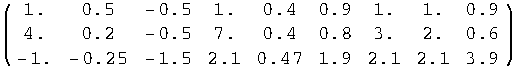
\includegraphics{refHmat.pdf}}}\intertext{with $\psi_c=\psi_\epsilon=0, \,\,  \psi_z=I$.
the series representation requires that the linear model
have a unique stable solution.}
  B=
\vcenter{\hbox{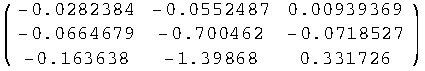
\includegraphics{refBmat.pdf}}}\\
\phi=
\vcenter{\hbox{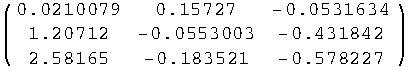
\includegraphics{refPhimat.pdf}}}\\
F=
\vcenter{\hbox{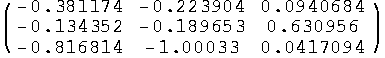
\includegraphics{refFmat.pdf}}}
\end{gather} 

\end{frame}
\begin{frame}
  

\begin{figure}
  \centering
\includegraphics[width=1.1in]{piPath.pdf}
\includegraphics[width=1.1in]{oscillPath.pdf}
\includegraphics[width=1.1in]{pseudoPath.pdf}

\includegraphics[width=2in]{theZs.pdf}
\includegraphics[width=2in]{arbTruncErr.pdf}  
\caption{RBC Truncation Error Bound Versus Actual}
  \caption{State Variables and the  z's Corresponding to  $x_{-1}=(1,2,3),\epsilon=(2,1,2)$} \label{arbFig}
\end{figure}

\end{frame}



  \begin{frame}
    
\frametitle{ RBC Model Example}
  See for example\cite{Maliar2005}
 \begin{gather*}
   \max\left \{  u(c_t^t) + E_t \sum_{\tau=t}^\infty \beta \delta^{\tau+1-t}u(c_{\tau+1}^t)\right \}\\
c_\tau^t + k_\tau^{t+1}=(1-d)k_\tau^{t-1} + \theta_\tau f(k_\tau^{t-1})\\
f(k_\tau^{t-1})= k_\tau^\alpha
\intertext{with first order conditions}
\frac{1}{c_t^{\eta}}=\alpha \delta k_{t}^{\alpha-1} E_t \left (\frac{\theta_{t}}{c_{t+1}^\eta} \right ) \\
c_t + k_t=\theta_{t-1}k_{t-1}^\alpha \\
 \theta_t =\theta_{t-1}^\rho e^{\epsilon_t}\label{rbcSys}
 \end{gather*}

  \end{frame}

\begin{frame}
\frametitle{for $\eta=\delta=1$}


\begin{gather}
\frac{1}{c_t}=\alpha \delta k_{t}^{\alpha-1} E_t \left (\frac{\theta_{t}}{c_{t+1}} \right ) \\
c_t + k_t=\theta_{t-1}k_{t-1}^\alpha \\
\theta_t =\theta_{t-1}^\rho e^{\epsilon_t}\label{rbcSys}
\intertext{and there is a closed form solution}
  k_{t}= \alpha \delta \theta_{t} k_{t-1}^\alpha.\label{soln}\\
c_t=  (1-\alpha \delta) \theta_{t} k_{t-1}^\alpha
\end{gather}
  \end{frame}
\begin{frame}


For mean zero iid $\epsilon_t$ we can easily compute a family of trajectories like \refeq{fFamily}
\begin{gather}
  \begin{bmatrix}
c_{t+s}(k_{t-1},\theta_t,\epsilon_t)\\k_{t+s}(k_{t-1},\theta_t,\epsilon_t)    \\ \theta_{t+s}(\theta_{t-1},\theta_t,\epsilon_t)    
  \end{bmatrix}
\intertext{with conditional mean converging over time to }
  \begin{bmatrix}
    c_{ss}\\k_{ss}
  \end{bmatrix}=
  \begin{bmatrix}
\nu^\alpha-\nu\\ \nu
  \end{bmatrix}\intertext{where}
\nu= \alpha ^{\frac{1}{1-\alpha }} \delta ^{\frac{1}{1-\alpha }}
\end{gather}

\end{frame}



  \begin{frame}
    \frametitle{Truncations Errors: Arbitrary System and Linearized System}


\begin{figure}[H]
  \centering
\includegraphics[width=2in]{arbTruncErrSimp.pdf}  
\includegraphics[width=2in]{TruncErrSimp.pdf}  
\caption{RBC Model Series Truncation Error Bounds Versus Actual}
  \caption{ $x_{-1}=( {{0.2}, {0.18}, {1.1}}), \epsilon=0.01$} \label{arbFig}
\end{figure}


  \end{frame}





\begin{frame}
\frametitle{Consider  models that can be written in  the following form}


\begin{gather}
  h_i(x_{t-1},x_{t},x_{t+1},\epsilon_t)=h^{det}_{io}(x_{t-1},x_{t},\epsilon_t)+\\ \sum_{j=1}^{p_i} [h^{det}_{ij}(x_{t-1},x_{t},\epsilon_t)h^{nondet}_{ij}(x_{t},x_{t+1},\epsilon_t)]=0
\end{gather}

\begin{itemize}
\item models where expectations are computed at time t, $\epsilon_t$  known
\item this specification allows use of auxiliary variables for 
accurately computing expected values of nonlinear quatities.
\item if expected lagged values shocks known then deterministic system in L variables
\end{itemize}

\end{frame}


\begin{frame}
\frametitle{the example  model }
\label{sec:simple-rbc-model-ext} can be written as
\begin{gather}
h_{10^{det}}(\cdot)=\frac{1}{c_t},\,\,
h_{11}^{det}()=\alpha \delta k_{t}^{\alpha-1} ,\,\,
h_{11}^{nondet}(\cdot)=E_t \left (\frac{\theta_{t+1}}{c_{t+1}} \right )\\
h_{20}^{det}(\cdot)=c_t + k_t-\theta_tk_{t-1}^\alpha,\,\,
h_{21}^{det}(\cdot)=0\\
h_{30}^{det}(\cdot)=\ln \theta_t -(\rho \ln \theta_{t-1} + \epsilon_t),\,\,
h_{31}^{det}(\cdot)=0
\end{gather}

\end{frame}

\begin{frame}
  \frametitle{Some definitions}

{\small

  \begin{description}
  \item[$\numX$-Dimensional Linear Reference Model] \ 

$\linMod \equiv \linModMats$ A linear model with state space of dimension
$\numX$ and unique solutions converging 
to some steady state
  \item[Augmented Decision Rule Function(\ADR)]  \ 
$\xzFunc: \xzFuncSig$ \\
 A function of $
\begin{bmatrix}
  x_{t-1}\\\epsilon_t
\end{bmatrix}
$ providing an approximation 
for $\begin{bmatrix}
  x_t\\z_t
\end{bmatrix}$
  \item[Augmented Decision Rule Unconditional Expectation Function(\ADRUE)] 

$\XZFunc: \xzFuncGuessSig$ \\ A function of $x_t$ providing an approximation 
for the unconditional expectation  
$\uncnxpt{\begin{bmatrix}
  x_{t+1}\\z_{t+1}
\end{bmatrix}}{x_t}\equiv  \uncnxpt{\xzFunc(x_t,\epsilon_{t+1})}{x_t}$

  \end{description}

}

\end{frame}




\begin{frame}

{\small
  \begin{gather}
  \xzFuncGuess^k \left (
  \begin{bmatrix}
    x_{t-1} \\\epsilon_t
  \end{bmatrix}; \linMod,\xguss
\right )=
  \begin{bmatrix}
    x_{t-1}\\ x_t\\ \xtpguss
  \end{bmatrix}\\
x_t= \sumLinPart + \sumZPartZero +\\  \sumZPartPos(\xguss)  \label{seriesForm}\\ 
\xtpguss=\XZFunc^{k-1}(\xguss) = \sumZPartZero +  \sumZPartPos(\xguss)
  \end{gather}
}
\end{frame}

\begin{frame}
\frametitle{Perfect Foresight}




\begin{gather}
\XZFunc^{k}(x)=     \mathcal{H}^{PF}[\xzFunc^{k}(x,\epsilon_{t+T-k+1})]=\\
\XZFunc^{k}(x)=\EsumLinPart +   \EsumZPartZero\\
 \XZFunc^{k}(x)=\EsumLinPart + \EsumCapZPart{PF}
\end{gather}

\end{frame}
\begin{frame}
  
 \frametitle{Rational Expectations}

 \begin{gather}
 \XZFunc^{k}(x)=     \mathcal{H}^{RE}[\xzFunc^{k}(x,\epsilon_{t+T-k+1})]=
 \expct{\xzFunc^{k}(x,\epsilon_{t+T-k+1})}\\
  \XZFunc^{k}(x)=\EsumLinPart + \EsumZPartEpsilon\\
 \XZFunc^{k}(x)=\EsumLinPart + \EsumCapZPart{RE}
 \end{gather}

\end{frame}


\begin{frame}[fragile]

{\small
%Choose a linear reference  model, $\linMod$, of dimension $\numX$,
%the number of terms for the series $\numTerms$  and interpolation/collocation points,  $\thePts \equiv \thePoints$.
%Choose an initial \ADRUE,  $\XZFunc^0$
}

{\small
  \begin{algorithm}[H]{Compute the \ADR\ $\xzFunc^k(\xtmEpsArg)$ to improve the \ADRUE, $\XZFunc^{k}$}\\
\SetKwInOut{Input}{input}
\SetKwInOut{Output}{output}
\Input{$\linMod, \XZFunc^k, \numTerms, \thePts$}
%\For{(\xtmEpsArg) \in \thePts }{ xx}
\For{$(\xtmEpsArg) \in \thePts$}{
initialize $\xgusst{t}= \XZFunc^k(x_{t-1})$\;
\Repeat{$\xlst{t} = \xnxt{t}$}
{$\xlst{t}=\xgusst{t}$\\
use $\XZFunc^{k}$ to recursively compute 
$\left \{
\begin{bmatrix}
\xgusst{t+1}\\\zgusst{t+1}
\end{bmatrix}
\cdots
\begin{bmatrix}
\xgusst{t+\numTerms-1}\\  \zgusst{t+\numTerms-1}
\end{bmatrix}
\right \}$\;
use \refeq{seriesForm} to compute $\xzFuncGuess(\xtArg;\xgusst{t})$\;
solve $\eqnFunc(\xzFuncGuess(\xtArg;\xgusst{t}))$ to determine $\xnxt{t}, \znxt{t}$\;
$\xgusst{t}=\xnxt{t}$\;
}
}
$\xzFunc^{k+1}(\xtmEpsArg)\,\,  \forall \, (\xtmEpsArg)\in \thePts \Rightarrow \XZFunc^{k+1} $\;
\Output{$\XZFunc^{k+1}$}
%$\XZFunc^{k+1}(\xtArg)=\int \xzFunc^{k+1}(\xtArg,\epsilon) d\epsilon$

\end{algorithm}
}

\end{frame}

\begin{frame}
  \frametitle{Algorithm Operation Counts}
  \begin{description}
  \item[Solve Deterministic Problem]
    \begin{description}
    \item[Expectation Computations] 
    \item[Function Generation] 
    \end{description}
  \end{description}
\end{frame}



\begin{frame}
  \frametitle{RBC Known Solution Truncation Error }
  \begin{description}
  \item[Deterministic Solution] 
  \item[Expectation Computation] 
\item[Function Generation]
  \end{description}

\end{frame}


\begin{frame}
  \frametitle{RBC Unknown Solution Truncation Error }
  \begin{description}
  \item[Deterministic Solution] 
  \item[Expectation Computation] 
\item[Function Generation]
  \end{description}

\end{frame}


\begin{frame}
  \frametitle{RBC Occasionally Binding Constraints Truncation Error }
  \begin{description}
  \item[Deterministic Solution] 
  \item[Expectation Computation] 
\item[Function Generation]
  \end{description}

\end{frame}


\begin{frame}
  \frametitle{RBC Regime Switching Truncation Error }
  \begin{description}
  \item[Deterministic Solution] 
  \item[Expectation Computation] 
\item[Function Generation]
  \end{description}

\end{frame}



\begin{frame}
  \frametitle{RBC Occasionally Binding Constraints and Regime Switching  Truncation Error }
  \begin{description}
  \item[Deterministic Solution] 
  \item[Expectation Computation] 
\item[Function Generation]
  \end{description}

\end{frame}


\begin{frame}[fragile]
  \frametitle{some cat for functions}
  \begin{tikzcd}
    A \arrow [ r,"f"]
\arrow[dr,swap,"g\circ f"]&
B \arrow[dr,"g\circ h"]
\\{}&
C \arrow[r,swap,"h"]
&
D
  \end{tikzcd}
\end{frame}



% \begin{frame}
% \frametitle{Program Signatures}
% \label{sec:program-listings}
% \begin{tabular}{|l|c|}
% \hline
% Number of $x_t$ variables&$\numX$\\
% \hline
% Number of $z_t$ variables&$\numZ$\\
% \hline
% Number of $\epsilon_t$ variables&$\numEps$\\
% \hline
% Number of regimes variables&$\numR$\\
% \hline
% Number of recursive iterations&$\numIters$\\
% \hline
% Interpolation Grid Specification&$\dstSpec$\\
% \hline
% Shock Distributions  Specification&$\dstSpec$\\
% \hline
% The Linear Reference Model&$\linMod\equiv\linModMats$\\  
% \hline
% Model Equation Function&$\eqnFuncSig$\\
% \hline
% \end{tabular}

% \end{frame}


% \begin{frame}
% \frametitle{Solvers}
% {\small
% \begin{itemize}
% \item genFRFunc  -- Mathematica FindRoot for equations alone
% \item genNSFunc  -- Mathematica NSolve for equations and inequalities
% \end{itemize}
% }
%   \begin{gather}
% \genSlvr:\{\numX,\numEps,\numZ\}\times \xzFunc\times \eqnFunc    \rightarrow\slvr \intertext{ where }
% \xzFunc(\xguss):\xzFuncGuessSig\\
% \eqnFunc:\eqnFuncSig\\
%     \slvr : \solverSig\\
% \slvr \left (
% \begin{bmatrix}
%   x_{t-1}\\\epsilon
% \end{bmatrix}
% ;\xguss \right ) \rightarrow
% \begin{bmatrix}
%   x_t(\xguss)\\z_t(\xguss)
% \end{bmatrix}
%   \end{gather}
% \end{frame}

% \begin{frame}
%   \frametitle{FixedPoint for $\xguss$}
% {\small
% \begin{gather*}
% \genXGFP:\genSlvr\times \linMod \times \{  \XZFunc, \numTerms\} \times \eqnFunc    \rightarrow\\ 
% \xgFP : \frfpnsFuncSig\\ \intertext{where}
% \XZFunc : \bigXFuncSig\\
% \eqnFunc: \eqnFuncSig \intertext{so that}
% \xgFP \left (
%   \begin{bmatrix}
%     x_{t-1}\\ \epsilon_t
%   \end{bmatrix}
% \right )\rightarrow
% \begin{bmatrix}
%   x_{t}\\z_{t}
% \end{bmatrix}
% \end{gather*}
% }
% \begin{itemize}
% \item $\xgFP$ is a function that for a given $\XZFunc^k$ provides $
% l  \begin{bmatrix}
%     x_{t}\\ z_t
%   \end{bmatrix}$ consistent with a $x_{t-1}, \epsilon_t$

% \end{itemize}

% \end{frame}

% \begin{frame}
% \frametitle{genLilXkZkFunc}
% \label{sec:genlilxkzkfunc}
% \begin{gather}
% \xzFunc^k(x_{t-1},\epsilon_t):\xzFuncGuessSig\\
% \XZFunc^k(x_{t-1})=\expct{ \xzFunc^k(x_{t-1},\epsilon_t):\xzFuncGuessSig}\\
% \XZFunc^k(x_{t-1}):\bigXFuncSig\\
% \xzFunc^{k+1}(x_{t-1},\epsilon_t):\xzFuncGuessSig\\
%   \Gamma_1(\linMod,\{\XZFunc^k,\numTerms\},\xguss)
% \end{gather}
% {\small
% \begin{gather*}
% \linMod \times \{  \bigXFuncSig, k \} \times \Rn{(\numX+\numEps)} \rightarrow
% \xzFuncGuessSig
% \end{gather*}
% }
% \end{frame}


% % \begin{frame}
% %   \begin{algorithm}{Improve Augmented Approximate Decision Rule н$\xzFunc(\xNow{})$}
% %     \begin{algorithmic}
% % x      
% %     \end{algorithmic}
% %   \end{algorithm}
% % \end{frame}



% \begin{frame}
% \frametitle{genFRFunc,genNSFunc}
% \label{sec:genfrfunc}
%   \begin{itemize}
%   \item use accuracy requirement and truncation error formula to determine number of terms
%   \item begin with the linear reference model to construct $xz^0$ and $XZ^0$
%   \item construct an initial guess for a next $xz^{k+1}$ func which embeds
% for any given $(x_{t-1},\epsilon_t)$ a guess for $x_t$ 
%   \item use the solver to solve for tentative $z_t$ and consequently 
% a tentative $x_t$ use this as a new guess.  
% \item Repeat until guess doesn't change producing  a new $xz^{k+1}$
% \item Compute $XZ^{k+1}$
% \item Repeat above process until $xz$ and consequently $XZ$ don't change
%   \end{itemize}
% \end{frame}

% \begin{frame}
  
% \end{frame}

% \begin{frame}
% \frametitle{genFRFunc,genNSFunc}
% \begin{gather*}
% \{\numX,\numEps,\numZ\}\times(\xzFuncGuessSig)\times (\eqnFuncSig)    \rightarrow\\
% \frfpnsFuncSig
% \end{gather*}
% \end{frame}

% \begin{frame}
% \frametitle{genFPFunc}
% \label{sec:genfpfunc}
% \begin{gather*}
% \linMod \times \{  \bigXFuncSig, k \} \times (\eqnFuncSig)    \rightarrow\\ 
% \frfpnsFuncSig
% \end{gather*}

% \end{frame}

% \begin{frame}
% \frametitle{genXZREInterpFunc}
% \label{sec:genfpfunc}
% \begin{gather*}
% \{\numX,\numEps,\numZ\}\times(\xzFuncGuessSig)\times \grdSpec \times  \dstSpec   \rightarrow\\
% \bigXFuncSig
% \end{gather*}



% \end{frame}
% \begin{frame}
% \frametitle{doIterREInterp}
% \label{sec:doiterreinterp}

% \begin{gather*}
%   \linMod \times 
% w\{(\xzFuncGuessSig)_1,\ldots,(\xzFuncGuessSig)_{\numR}\}  \\
%  \times (\eqnFuncSig ) \times \grdSpec \times \dstSpec \rightarrow\\
% \{\frfpnsFuncSig, \{(\xzFuncGuessSig)_1,\ldots,(\xzFuncGuessSig)_{\numR}\}\}
% \end{gather*}



% \end{frame}
% \begin{frame}
% \frametitle{nestIterREInterp}
% \label{sec:nestiterreinterp}



% \begin{gather*}
%   \linMod \times 
% \{(\xzFuncGuessSig)_1,\ldots,(\xzFuncGuessSig)_{\numR}\}  \\
%  \times (\eqnFuncSig ) \times \grdSpec \times \dstSpec \times \numIters \rightarrow\\
% \{\frfpnsFuncSig, \{(\xzFuncGuessSig)_1,\ldots,(\xzFuncGuessSig)_{\numR}\}\}
% \end{gather*}



% \end{frame}
% \begin{frame}
% \frametitle{genLilXkZkRegimeFuncs}
% \label{sec:genlilxkzkregimefunc}
% {\small
% \begin{gather*}
% \linMod \times \{(\{  \bigXFuncSig, k_i \})_{k_i=1},\ldots,(\{  \bigXFuncSig, k_i \})_{k_i=\numR}\} \times\\ \Rn{(\numX+\numEps)} \rightarrow\\
% \{(\lilXRegimeFuncSig)_1,\ldots,(\xzFuncGuessSig)_{\numR}\}
% \end{gather*}
% }





% \end{frame}
% \begin{frame}
% \frametitle{genFRRegimeFuncs, genNSRegimeFuncs}
% \label{sec:genfrregimefunc}



% {\small
% \begin{gather*}
% \{\numX,\numEps,\numZ\}\times\\
% \{(\lilXRegimeFuncSig)_1,\ldots,(\xzFuncGuessSig)_{\numR}\}  \\
%  \times (\eqnRegimeFuncSig )\rightarrow\\
% \frfpnsRegimeFuncSig
% \end{gather*}
% }








% \end{frame}
% \begin{frame}
% \frametitle{genFPRegimeFuncs}
% \label{sec:genfpregimefunc}




% {\small
% \begin{gather*}
% \{\numX,\numEps,\numZ\}\times\\
% \{(\lilXRegimeFuncSig)_1,\ldots,(\xzFuncGuessSig)_{\numR}\}  \\
%  \times (\eqnRegimeFuncSig )\rightarrow\\
% \frfpnsRegimeFuncSig
% \end{gather*}
% }




% \end{frame}
% \begin{frame}
% \frametitle{genXZREInterpRegimeFuncs}
% \label{sec:genfpfunc}
% \begin{gather*}
% \{\numX,\numEps,\numZ\}\times(\xzFuncGuessSig)\times \dstSpec \times  \expctSpec   \rightarrow\\
% \frfpnsFuncSig
% \end{gather*}



% \end{frame}
% \begin{frame}
% \frametitle{doIterREInterpRegime}
% \label{sec:doiterreinterp}

% \begin{gather*}
%   \linMod \times 
% w\{(\lilXRegimeFuncSig)_1,\ldots,(\xzFuncGuessSig)_{\numR}\}  \\
%  \times (\eqnRegimeFuncSig ) \times \grdSpec \times \dstSpec \rightarrow\\
% \{\frfpnsRegimeFuncSig, \{(\lilXRegimeFuncSig)_1,\ldots,(\xzFuncGuessSig)_{\numR}\}\}
% \end{gather*}



% \end{frame}
% \begin{frame}
% \frametitle{nestIterREInterpRegime}
% \label{sec:nestiterreinterp}



% \begin{gather*}
%   \linMod \times 
% \{(\lilXRegimeFuncSig)_1,\ldots,(\xzFuncGuessSig)_{\numR}\}  \\
%  \times (\eqnRegimeFuncSig ) \times \grdSpec \times \dstSpec  \times \numIters \rightarrow\\
% \{\frfpnsRegimeFuncSig, \{(\lilXRegimeFuncSig)_1,\ldots,(\xzFuncGuessSig)_{\numR}\}\}
% \end{gather*}


% \end{frame}
% \begin{frame}
% \frametitle{Representing a Path}

% \end{frame}
% \begin{frame}
% \frametitle{Representing a Family of Paths}

% \end{frame}
% \begin{frame}
% \frametitle{Useful Properties of Series Solution}

% \begin{itemize}
% \item linear sum of functions
% \item far away points matter less
% \item Bounds on errors
% \end{itemize}



% \end{frame}
% \begin{frame}
% \frametitle{An RBC Model Example}
% \end{frame}
% \begin{frame}
% \frametitle{Known Solution: Conditional Expectations Path}
% \begin{itemize}
% \item can easily compute series
% \item algorithm can recover known solution
% \end{itemize}


% \end{frame}
% \begin{frame}
% \frametitle{UnKnown Solution: Conditional Expectations Path}
% \begin{itemize}
% \item can discover unknown solutions
% \end{itemize}



% \end{frame}
% \begin{frame}
% \frametitle{Occassionally Binding Constraints}
% \begin{itemize}
% \item can discover unknown solutions
% \end{itemize}



% \end{frame}
% \begin{frame}
% \frametitle{Regime Switching}
% \begin{itemize}
% \item can discover unknown solutions
% \end{itemize}


% \end{frame}
% \begin{frame}
% \frametitle{Regime Switching with Occassionally Binding Constraints}
% \begin{itemize}
% \item can discover unknown solutions
% \end{itemize}

% \end{frame}
% \begin{frame}
% \frametitle{Future Directions}
% \end{frame}
\begin{frame}
  \frametitle{Future Directions}
  \begin{itemize}
  \item Using Parallelization to Solve a Macroeconomic Model: A Parallel Parameterized Expectations Algorithm
Michael Creel
  \item frbus implications/.,mbnvnvbm,.n/.''.jj'.'j;'jjjjj'j;.'''
  \item bound other people's solutions, compare to bound Euler errors
  \item show can determin number series terms then accracy depends on number of nodes
  \item should normalize h since just scaling up moves bounds around
  \item can precompute z's for exogenous backward looking quantities
  \item evaluation points for XZ and xz need not be the same
  \item model solutions with closed form values produce right series stable difference equations?
  \item add points for interpolation outside range
  \item filter fixedpoint and findroot failures
  \item add list of solvers to ``try'' if there are falures
  \item record performance of solvers using sow reap (functional?)
  \item Heterogeneous Agents Problems
  \item Convergence Properties
    \begin{itemize}
    \item no solution
    \item multiple solutions
    \end{itemize}
\item algorithmic details
  \begin{itemize}
 \item Smolyak nodes
 \item Judd Ergodic region
 \item F small eigenvalues
 \item Projection Methods
 \item Perturbation Methods for initial guess
  \end{itemize}
\item Insights for ``pruning''
  \end{itemize}
\end{frame}

\begin{frame}
  \frametitle{Bibliography}
  \bibliographystyle{plainnat}
\bibliography{anderson,files}

\end{frame}

\appendix


\end{document}
